\hsection{Violation:~Non-Key Attribute Transitively Depends on Primary Key}%
\FloatBarrier%
%
\begin{figure}%
\centering%
%
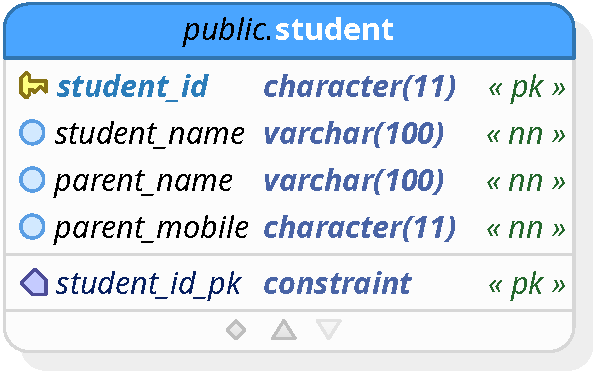
\includegraphics[width=0.56\linewidth]{\currentDir/studentViolation3nf}%
%
\caption{A table which stores data about students and their parents.}%
\label{fig:studentViolation3nf}%
\end{figure}%
%
\gitExec{\databasesCodeRepo}{.}{_scripts_/postgres.sh normalization/3nf/student/violation/generated_sql 01_violation_database_2001.sql}%
%
\gitSQL{\databasesCodeRepo}{normalization/3nf/student/violation/generated_sql/03_public_student_table_5071.sql}{3nf:violation:03_public_student_table_5071}{The generated \sql\ code for creating the table \sqlil{student} that violates the \pgls{3NF} based on \cref{fig:studentViolation3nf}.}%
\gitExec{\databasesCodeRepo}{.}{_scripts_/postgres.sh normalization/3nf/student/violation/generated_sql 03_public_student_table_5071.sql violation}%
%
\gitSQL{\databasesCodeRepo}{normalization/3nf/student/violation/insert.sql}{normalization:3nf:student:violation:insert}{%
Inserting some data into the table~\sqlil{student} in violation of the \pgls{3NF}.}%
\gitExec{\databasesCodeRepo}{.}{_scripts_/postgres.sh normalization/3nf/student/violation insert.sql violation}%
%
\gitSQLAndOutput{\databasesCodeRepo}{normalization/3nf/student/violation}{update.sql}{violation}{}{}{postgres.sh}{normalization:3nf:student:violation:update}{%
We noticed that the name of the father of Mr.~Bibbo, Mr.~Bibotto, and Ms.~Bibboba is actually Mr.~B{\"o}dd{\"o}, not Mr.~Boddo. %
To change it, we need to touch three records, which is a typical update anomaly.%
}%
%
%
In \cref{fig:studentViolation3nf}, we show a part of logical model which illustrates a \db\ table for storing information about students and their parents.
The table has five columns.
In the first column, we store the student~ID, which is the primary key.
In the second column we store the national Chinese~ID number~(中国公民身份号码).
This is not a key column, since the same person may enroll into more than one programme, maybe first do a BSc and then go for a Master's degree.
The column with the student name is also not a key and not necessarily unique.
For each student, we also store the name of one parent and their mobile phone number as a contact for emergencies.

This table is in the \pgls{1NF}, as there are neither compound attributes nor repeated groups.
It is also in the \pgls{2NF}, because there is no compound key and, hence, it is not possible that an attribute cound depend on a part of such a key only.
However, this table violates the \pgls{3NF}.
The attribute \sqlil{parent_name} is functionally dependent on the attribute \sqlil{parent_mobile}.
We can write~\funcDepb{\sqlil{parent_mobile}}{\sqlil{parent_name}}.
A mobile phone number is associated with a single person, hence there can only be one name for a given mobile phone number.
Both the parent mobile phone number and the parent name also depend on the primary key.
The transitive relationship \funcDepb{\sqlil{student_id}}{\funcDepb{\sqlil{parent_mobile}}{\sqlil{parent_name}}} exists.
And it violates the \pgls{3NF}.

Let us explore what consequences this has.
We first create the table by executing the script given in \cref{lst:3nf:violation:03_public_student_table_5071}.
Then we insert four student records into the \db\ using the script given in \cref{lst:normalization:3nf:student:violation:insert}.
There are four students, Mr.~Bibbo, Mr.~Bebbo, Mr.~Bibboto, and Ms.~Bibboba.
Their IDs are not important.
What is important is that Mr.~Bibbo, Mr.~Bibboto, and Ms.~Bibboba happen to be sibblings.
Their proud father is Mr.~B{\"o}dd{\"o}.

Now it happened that, being located in China, the teacher in the administrative office did not really know how to enter the letter~\inQuotes{\"o}.
So they chose, for the time being, to call the dad of the three kids simply Mr.~Boddo.
A few days later, the found a solution on how to enter the letter~\inQuotes{\"o}.
In order to fix the data, they created the script \cref{lst:normalization:3nf:student:violation:update}.

They use the mobile phone number~555\decSep444\decSep666\decSep77 of Mr.~B{\"o}dd{\"o} to identify him in the table.
To test this, the script it uses a \sqlilIdx{SELECT} statement to get the three student/parent name pairs associated with this mobile phone number.
The output of this command is as expected, so next they launch an \sqlilIdx{UPDATE} command.
The \sqlil{parent_name} is \sqlilIdx{SET} to~\sqlil{Böddö} for each record where \sqlil{parent_mobile = '55544466677'}.
The updated records are returned via the~\sqlilIdx{RETURNING} statement.
As we can see, three rows are affected.

So to change one piece of information, three rows needed to be touched.
This is a classical example of an update anomaly.
Similarly, if we would delete the records of Mr.~Bibbo, Mr.~Bibboto, and Ms.~Bibboba, all the data about their dad would disappear as well.
If we had some reason to retain this data in that case, then that would be an deletion anomaly.
Finally, since we cannot insert the data of a parent without inserting data about a student first, that would be an insertion anomaly.

Well, the real problem in this example is the update anomaly, the other two anomalies would not be an issue in this specific scenario.
What is an issue, though, is that we again need to enter the same information several times.
This very much increases the probability of typos and other errors that could lead to data inconsistency.

For example, it could have well been possible that the information about the students were entered by different teachers.
Then, maybe one teacher would know how to enter an~\inQuotes{\"o} while another one would just use an~\inQuotes{o}.
And baam, our data would be inconsistent, as we would have same parent with two different names in our system.%
%
\FloatBarrier%
\endhsection%
%
